
%(BEGIN_QUESTION)
% Copyright 2009, Tony R. Kuphaldt, released under the Creative Commons Attribution License (v 1.0)
% This means you may do almost anything with this work of mine, so long as you give me proper credit

Connect a loop-powered temperature transmitter (4-20 mA output) to a DC voltage source and a meter such that the meter will indicate a increasing signal when the temperature-sensing element is heated.  All electrical connections must be made using a terminal strip (no twisted wires, crimp splices, wire nuts, spring clips, or ``alligator'' clips permitted).

This exercise tests your ability to properly connect power to a loop-powered temperature transmitter, connect multiple batteries together to achieve the required total supply voltage, identify different types of thermocouples and RTDs, properly connect either a thermocouple or an RTD to the transmitter, condition the electrical signal (if necessary) so the meter can properly register it, properly connect an analog meter into the circuit, and use a terminal strip to organize all electrical connections.

$$\includegraphics[width=15.5cm]{i03775x01.eps}$$

\vskip 10pt

The following components and materials will be available to you during the exam: assorted 2-wire 4-20 mA temperature {\bf transmitters} calibrated to ranges inclusive of room temperature ; an assortment of {\bf thermocouples} and {\bf RTDs} ; {\bf terminal strips} ; lengths of {\bf hook-up wire} ; 250 $\Omega$ (or approximate) {\bf resistors} ; analog {\bf meters} ; {\bf battery clips} (holders).

\vskip 10pt

You will be expected to supply your own screwdrivers and multimeter for assembling and testing the circuit at your desk.  The instructor will supply the battery(ies) to power your circuit when you are ready to see if it works.  Until that time, your circuit will remain unpowered.

\vskip 10pt

\noindent
{\bf Meter options} (instructor chooses): \hskip 20pt \underbar{\hskip 20pt} Voltmeter (1-5 VDC) \hskip 20pt \underbar{\hskip 20pt} Ammeter (4-20 mA)

\vskip 10pt

\noindent
{\bf Sensor type} (instructor chooses): \hskip 20pt \underbar{\hskip 20pt} Thermocouple \hskip 20pt \underbar{\hskip 20pt} RTD

\vfil

Study reference: the ``Analog Electronic Instrumentation'' chapter of {\it Lessons In Industrial Instrumentation}, particularly the sections on loop-powered transmitters and current loop troubleshooting.  Also, the ``Continuous Temperature Measurement'' chapter of the same textbook, particularly the sections on thermocouples and RTDs.

\underbar{file i03775}
%(END_QUESTION)





%(BEGIN_ANSWER)


%(END_ANSWER)





%(BEGIN_NOTES)


%INDEX% Mastery exam performance exercise (circuit), temperature transmitter

%(END_NOTES)


